
%%%%%%%%%%%%%%%%%%%%%%% file typeinst.tex %%%%%%%%%%%%%%%%%%%%%%%%%
%
% Template author: Mauricio Matamoros
% Updated: July 3, 2017
% Contact: mauricio@robocupathome.org
%
% This is the LaTeX source for the TDPTemplate using
% the LaTeX document class 'llncs.cls' Springer LNAI format
% used in the RoboCup Symposium submissions.
% http://www.springer.com/computer/lncs?SGWID=0-164-6-793341-0
%
% It may be used as a template for your own TDP - copy it
% to a new file with a new name and use it as the basis
% for your Team Description Paper
%
% NB: the document class 'llncs' has its own and detailed documentation, see
% ftp://ftp.springer.de/data/pubftp/pub/tex/latex/llncs/latex2e/llncsdoc.pdf
%
% Remark: Last page with specs won't be included in Camera ready TDP's.
%
%%%%%%%%%%%%%%%%%%%%%%%%%%%%%%%%%%%%%%%%%%%%%%%%%%%%%%%%%%%%%%%%%%%
%
% TU/e update: 27 oct 2017 - HvR

\documentclass[runningheads,a4paper]{llncs}
%\usepackage[left=48mm,right=46mm]{geometry}
%\usepackage[left=32mm,right=31mm]{geometry}

\usepackage[utf8]{inputenc}
\usepackage{amssymb}
\setcounter{tocdepth}{3}
\usepackage{url}
\usepackage{float}
\usepackage{amsmath}
\usepackage{graphicx}
\usepackage{wrapfig}
\usepackage{fancyhdr}
%\usepackage{titling}       % not used, messes up the titlepage!
%\usepackage{lipsum}  		% a garbage package you don't need except to create examples.

\newcommand{\robospecs}{%
	\newpage%
	\pagenumbering{gobble}%
	\pagestyle{fancy}%
	\fancyhf{}%
	\chead{$|$}
	\rhead{\footnotesize Robot Description}%
	\lhead{\footnotesize Tech United Eindhoven}%
	\rfoot{Robot software and hardware specification sheet}%
}

\newcommand{\BnL}[1][1em]{ 
\includegraphics[width=#1]{images/bnl.jpg} } 

% added HvR - 27oct2017 - from last year's (2017) template
\usepackage[english]{babel}	% input language for hyphens
\usepackage{listings}
\usepackage{enumitem}
%\usepackage{hyperref}      % not used, messes up almost all the figures!
\usepackage{booktabs}   	% For tables (toprule, midrule, bottomrule)

\setlength{\belowcaptionskip}{-10pt}

%%%%%%%%%%%%%%%%%%%%%%%%%%%%%%%%%%%%%%%%%%%%%%%%%%%%%%%%%%%%%%%%%%%
% *** PATHS ***
\makeatletter
\def\input@path{{Figures/}		
				}
\makeatother
\graphicspath{{Figures/}
				}
%%%%%%%%%%%%%%%%%%%%%%%%%%%%%%%%%%%%%%%%%%%%%%%%%%%%%%%%%%%%%%%%%%%

%%%%%%%%%%%%%%%%%%%%%%%%%%%%%%%%%%%%%%%%%%%%%%%%%%%%%%%%%%%%%%%%%%%

% Acronym definitions
\usepackage[acronym]{glossaries}
\newacronym{ed}{ED}{Environment Descriptor}
\newacronym{amcl}{AMCL}{Adaptive Monte Carlo Localization}
\newacronym{gui}{GUI}{Graphical User Interface}
%\newacronym{spl}{SPL}{Standard Platform League}
\newacronym{fcfg}{FCFG}{feature context free grammar}
\newacronym{ros}{ROS}{Robot Operating System}
\newacronym{wire}{WIRE}{World Information for Robotic Environments}
\newacronym{cnn}{CNN}{Convolution Neural Networks}

% shorthand definitions
\newcommand{\eg}{\emph{e.g.}}						% Exemplum gratia
\newcommand{\goal}{\mathcal{G}}						% Goal area
\newcommand{\goallc}{\mathcal{G}_{\mathrm{lc}}}		% Subset of goal area with costs below threshold cmin
\newcommand{\goalhc}{\mathcal{G}_{\mathrm{hc}}}		% Subset of goal area with costs above threshold cmin
\newcommand{\ie}{\emph{i.e.}}						% Id est
%%%%%%%%%%%%%%%%%%%%%%%%%%%%%%%%%%%%%%%%%%%%%%%%%%%%%%%%%%%%%%%%%%%

%%%%%%%%%%%%%%%%%%%%%%%%%%%%%%%%%%%%%%%%%%%%%%%%%%%%%%%%%%%%%%%%%%%%%%%%%%%%%%%%%%%%
%
% Title
%
%%%%%%%%%%%%%%%%%%%%%%%%%%%%%%%%%%%%%%%%%%%%%%%%%%%%%%%%%%%%%%%%%%%%%%%%%%%%%%%%%%%%
\begin{document}

\setlength{\headheight}{22pt}

\title{Tech United Eindhoven @Home \\2018 Team Description Paper}

\author{M.F.B.~van~der~Burgh , J.J.M.~Lunenburg, R.P.W.~Appeldoorn, R.W.J.~Wijnands,
T.T.G.~Clephas, M.J.J.~Baeten, L.L.A.M.~van~Beek, R.A.~Ottervanger,
S.~Aleksandrov, T.~Assman, K.~Dang, J.~Geijsberts, L.G.L.~Janssen,
H.W.A.M.~van~Rooy, A.T. Hofkamp and M.J.G.~van~de~Molengraft}

\institute{Eindhoven University of Technology,\\
Den Dolech 2, P.O. Box 513, 5600 MB Eindhoven, The Netherlands\\
\texttt{http://www.techunited.nl, techunited@tue.nl, https://github.com/tue-robotics}}

\authorrunning{Tech United Eindhoven}

%\author{Team Leader \and Team Members }
%\institute{[Institute name and direction here], \\
%\texttt{http://devoted-web-site.url}}

\maketitle
%%%%%%%%%%%%%%%%%%%%%%%%%%%%%%%%%%%%%%%%%%%%%%%%%%%%%%%%%%%%%%%%%%%%%%%%%%%%%%%%%%%%
%
% Abstract
%
%%%%%%%%%%%%%%%%%%%%%%%%%%%%%%%%%%%%%%%%%%%%%%%%%%%%%%%%%%%%%%%%%%%%%%%%%%%%%%%%%%%%
%
\begin{abstract}

%TODO list:\\
%DONE - Sound source localisation\\
%OpenPose\\
%Plans for this year?\\
%Clean-up of old stuff, reduce size. Increase size new parts.\\
%DONE - SERGIO in/out?\\
%ALMOST DONE - New template: \url{https://github.com/RoboCupAtHome/TDPTemplate/tree/template2018}\\
%              macro \robospecs does not work.....
%8 pages - DONE, excluding the robot specification pages.

%Video:\\
%Sound source localisation\\
%OpenPose\\
%Remove old stuff.\\
%Remove ugly video stuff\\


This paper provides an overview of the main developments of the Tech United Eindhoven RoboCup@Home team. Tech United uses an advanced world modeling representation system called the Environment Descriptor that allows straightforward implementation of localization, navigation, exploration, object detection \& recognition, object manipulation and robot-robot cooperation skills. Recent developments are improved object and people detection via deep learning methods, a generic GUI for different user levels, improved speech recognition, improved natural language interpretation and sound source localization.

\end{abstract}
%
%
%%%%%%%%%%%%%%%%%%%%%%%%%%%%%%%%%%%%%%%%%%%%%%%%%%%%%%%%%%%%%%%%%%%%%%%%%%%%%%%%%%%%%
%

\section{Introduction}
Tech United Eindhoven\footnote{\url{http://www.techunited.nl}} (established 2005) is the RoboCup student team of Eindhoven University of Technology\footnote{\url{http://www.tue.nl}} (TU/e), which joined the ambitious @Home League in 2011. The RoboCup@Home competition aims to develop service robots that can perform everyday tasks in dynamic and cluttered `home' environments.
The team has been awarded multiple world vice-champion titles in the Open Platform League (OPL) of the RoboCup@Home competition during previous years, and world champion titles in 2019 and 2022 in the Domestic Standard Platform League (DSPL). \\

\noindent Tech United Eindhoven consists of (former) PhD and MSc. students and staff members from different departments within the TU/e. The software base is developed to be robot independent, which means that the years of development on AMIGO and SERGIO are currently being used by HERO. Thus, a large part of the developments discussed in this paper have been optimized for years, whilst the DSPL competition has only existed since 2017\footnote{\url{https://athome.robocup.org/robocuphome-spl}}. All the software discussed in this paper is available open-source at GitHub\footnote{\url{https://github.com/tue-robotics}}, as well as various tutorials to assist with implementation. 


%Many parts of our software are interacting with the world-model. 
%Our world-model, \acrlong{ed}, is a database with 3D representations of objects. 
%This is described in section \ref{sec:ed}. 
%Other topics described in this paper are image recognition, pose detection, sound source localisation, Human-Robot interaction, Software sharing and community contributions.
%\\
%The previous years our focus has been on our own robots, AMIGO and SERGIO. 
%This year we are shifting our focus from our own robots, AMIGO and SERGIO to the Toyota HSR.
%This Team Description Paper is part of the qualification package for RoboCup 2019 in Sydney, Australia and describes the current status of the @Home activities of Tech United Eindhoven.


\section{\acrfull{ed}}
The TUe \acrfull{ed} is a \acrfull{ros} based 3D geometric, object-based world representation system for robots. In itself ED is database system that structures multi-modal sensor information and represents this in an object-based world representation that can be utilized for robot localisation, navigation, manipulation and interaction functions. See Figure \ref{fig:ed} for a schematic overview of ED. %\footnote{\acrshort{ed} is an evolution of \acrfull{wire}, that was created in the FP7 RoboEarth Project. Secondly, ED is utilized within the RoboCup @home competition (also read the \href{https://github.com/tue-robotics/team_description_paper/blob/master/Tech_United_At_Home_TDP_2015.pdf}{TU/e 2015 TDP} for RoboCup). More information, software, installation manual and tutorial can be found on \url{https://github.com/tue-robotics/ed}}
%An elaborate explanation, including tutorials are available at our GitHub website \footnote{\url{http://github.com/tue-robotics}}.
ED is used on our robots AMIGO and SERGIO in the open @Home league and will be used on the Toyota HSR in the DSPL. In previous years, developments have been focussed towards making ED platform independent. As a results ED had been used on the PR2 system, Turtlebot and Dr. Robot systems (X80).
\begin{figure}[h]
    %\vspace{-0.3cm}
	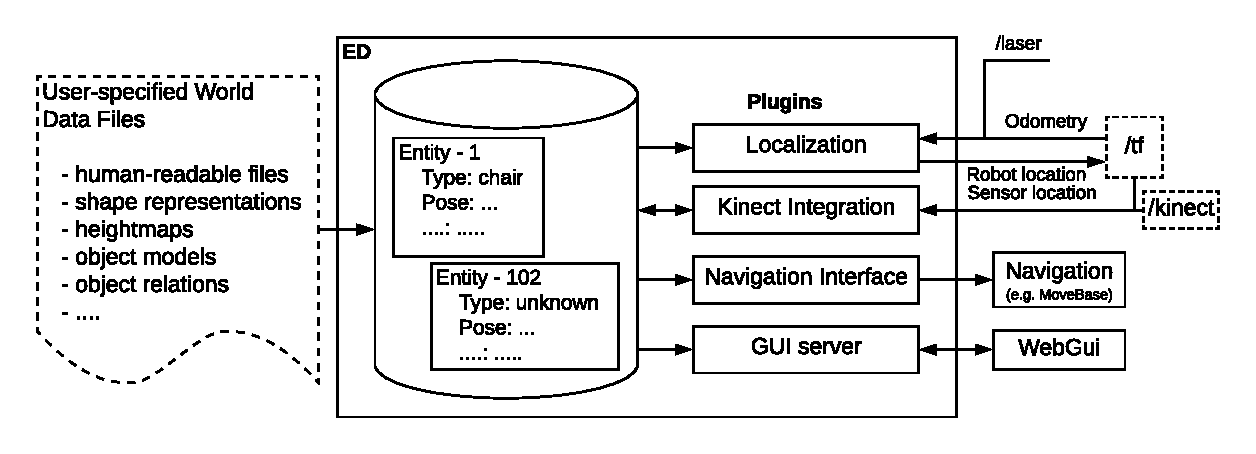
\includegraphics[width = 0.9\linewidth]{Figures/ed_overview}
    %\vspace{-1em}
	\caption{schematic overview of TUe Environment Descriptor.}
	\label{fig:ed}
    %\vspace{-0.5cm}
\end{figure}
ED is one re-usable environment description that can be used for a multitude of needed functionalities. Instead of having different environment representations for localization \acrfull{amcl}, navigation (MoveBase), manipulation (MoveIt!), interaction, etc.. An improvement in this single, central world model will reflect in the performances of the separate robot capabilities. It omits updating and synchronization of multiple world models. At the moment different ED plugins exist that enable robots to localize themselves, update positions of known objects based on recent sensor data, segment and store newly encountered objects and visualize all this through a web-based \acrshort{gui}, illustrated in Figure \ref{fig:gui_actions}.
\begin{figure}[h]
\centering
    %\vspace{-0.3cm}
	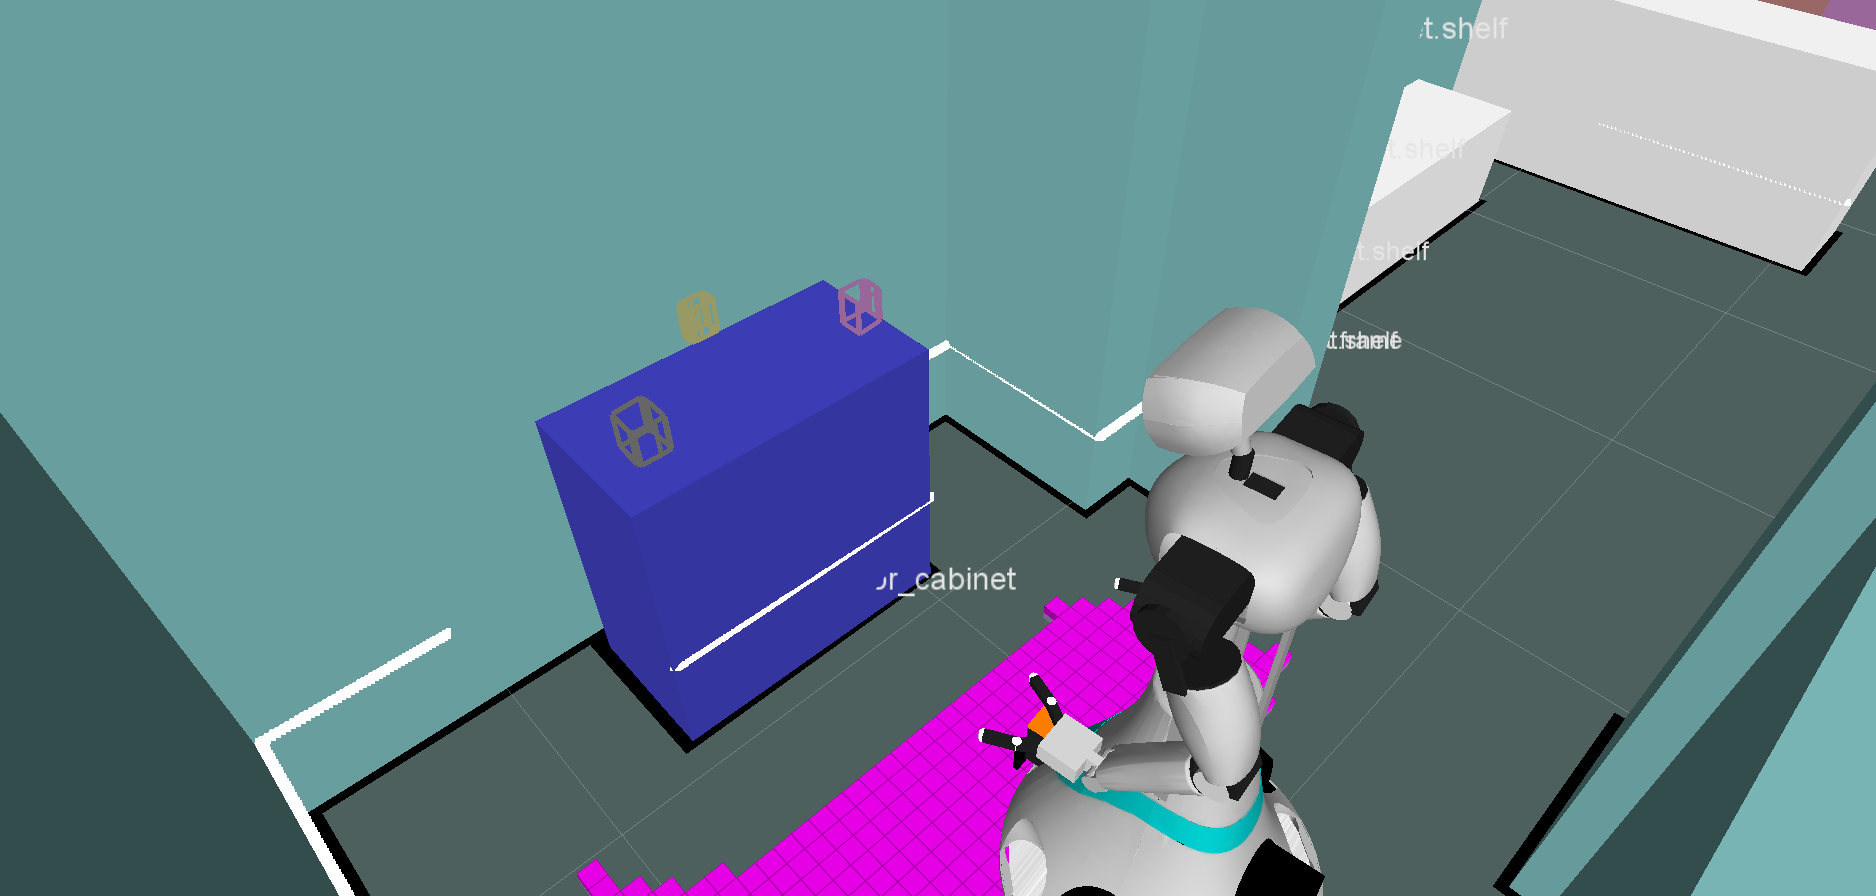
\includegraphics[width = 0.8\linewidth]{Figures/ed_segmentation}
    %\vspace{-0.5em}
	\caption{A view of the world model created with ED. The figure show the occupation grid as well as (unknown) objects recognized on top of the cabinet.}
	\label{fig:ed_segmentation}
    %\vspace{-0.5cm}
\end{figure}



\subsection{Localization, Navigation and Exploration}
The \emph{ed\_localization}\footnote{\url{https://github.com/tue-robotics/ed_localization}} plugin implements \acrshort{amcl} based on a 2D render of the central world model.
\\
With use of the \emph{ed\_navigation} plugin\footnote{\url{https://github.com/tue-robotics/ed_navigation}}, an occupancy grid is derived from the world model and published.
\\
With the use of the \emph{cb\_base\_navigation} package\footnote{\url{https://github.com/tue-robotics/cb_base_navigation}} the robots are able to deal with end goal constraints. The \emph{ed\_navigation} plugin allows to construct such a constraint w.r.t. a world model entity in \acrshort{ed}. This enables the robot to navigate not only to areas or entities in the scene, but to waypoints as well. Figure \ref{fig:ed_segmentation} also shows the navigation to an area.
% as illustrated by Figure \ref{fig:ed_navigation_constraints}.
Modified versions of the local and global ROS planners available within \emph{move\_base} are used.


\subsection{Object detection}
\subsubsection{Detection \& Segmentation}
ED enables integrating sensors through the use of the plugins present in the \textit{ed\_sensor\_integration} package. Two different plugins exist:
1. The \emph{laser\_plugin}: Enables tracking of 2D laser clusters. This plugin can be used to track dynamic obstacles such as humans.
2. The \emph{kinect\_plugin}: Enables world model updates with use of data from a RGBD camera. This plugin exposes several ROS services that realize different functionalities:
\begin{enumerate}[label=(\alph*)]
\item Segment: A service that segments sensor data that is not associated with other world model entities. Segmentation areas can be specified per entity in the scene. This allows to segment object `on-top-of’ or ‘in’ a cabinet. All points outside the segmented area are ignore for segmentation.
\item FitModel: A service that fits the specified model in the sensor data of a RGBD camara. This allows updating semi-static obstacles such as tables and chairs.
\end{enumerate}


The \emph{ed\_sensor\_integration} plugins enable updating and creating entities. However, new entities are classified as unknown entities. Classification is done in \emph{ed\_perception} plugin\footnote{\url{https://github.com/tue-robotics/ed_perception}} package. 

\subsection{Object grasping, moving and placing}
The system architecture developed for object manipulation is focused on grasping. In the implementation, its input is a specific target entity in \acrshort{ed}, selected by a Python executive and the output is the grasp motion joint trajectory.
Figure \ref{fig:grasping_pipeline} shows the grasping pipeline.
\begin{figure}[H]
    \centering
    %\vspace{-0.3cm}
	\includegraphics[width = 1\linewidth]{Figures/grasping_pipeline}
    %\vspace{-1em}
	\caption{Custom grasping pipeline base on \acrshort{ed}, MoveIt and a separate grasp point determination and approach vector node.}
	\label{fig:grasping_pipeline}
    %\vspace{-0.5cm}
\end{figure}
\noindent MoveIt! is used to produce joint trajectories over time, given the current configuration, robot model, \acrshort{ed} world model (for collision avoidance) and the final configuration.
%\acrshort{ed} provides collision meshes to MoveIt! so it can plan paths that avoid obstacles.
%Finally, the trajectories are sent to the reference interpolator which sends the trajectories either to the controllers or the simulated robot.
%The grasping pipeline is extended with an empty spot designator and grasping pose determination. The empty spot designator searches in an area, like `on-top-of'of the dinner table, for an empty spot to place an object by using the occupied area by other objects in this area.
The grasp pose determination uses the information about the position and shape of the object in \acrshort{ed} to determine the best grasping pose.
The grasping pose is a vector relative to the robot.
%An example of the determined grasping pose is shown in Figure \ref{fig:grasping_pose_determination}.
Placing an object is approached in a similar manner to grasping, except for that when placing an object, \acrshort{ed} is queried to find an empty placement pose.

%
%\begin{figure}[H]
%   \centering
%   %\vspace{-0.3cm}
%   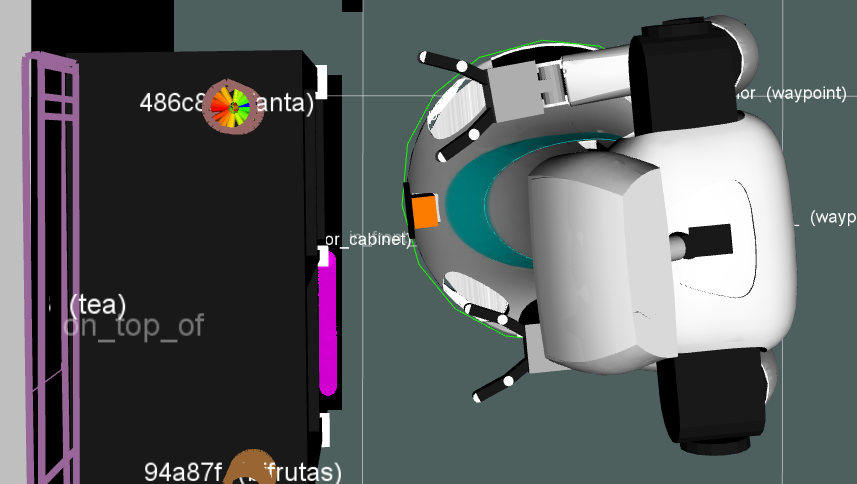
\includegraphics[width = 0.8\linewidth]{Figures/grasp_point_determination}
%    %\vspace{-1em}
%	\caption{Grasping pose determination result for a cylindric object with %TU/e built robot AMIGO. It is unpreferred to grasp the object from behind.}
%	\label{fig:grasping_pose_determination}
%    %\vspace{-0.5cm}
%\end{figure}


\section{Image Recognition}
In order the classify or train unknown entities, the ed\_perception plugin\footnote{\url{https://github.com/tue-robotics/ed_perception}} exposes ROS Services to classify the entities in the world model. The ed\_perception module interfaces with various image\_recognition nodes that apply state of the art image classification techniques based on \acrfull{cnn} illustrated in Figure \ref{fig:cnn}.
\begin{figure}[H]
    \centering
    %\vspace{-0.3cm}
	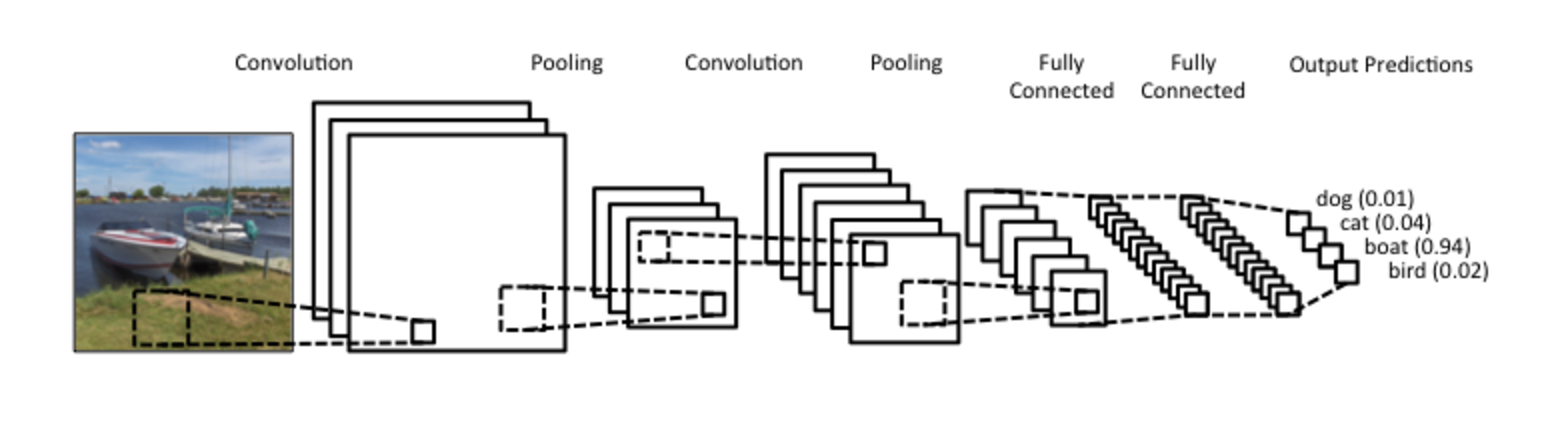
\includegraphics[width = 1\linewidth]{Figures/cnn}
    %\vspace{-1em}
    \caption{Illustration \acrfull{cnn} used in our object recognition nodes with use of Tensorflow.}
	\label{fig:cnn}
    %\vspace{-0.5cm}
\end{figure}

\subsection{Object recognition using Deep Learning}
Object recognition is done using Tensorflow: retraining the top-layer of a Inception V3 neural network. The top layers are retrained on a custom dataset using a soft-max top-layer that maps the image representation on a specified set of labels.
\\
In order to create a new training set for specific objects, the ed\_perception and the image\_recognition packages contain several tools for segmenting and annotating objects. Also tools for retraining neural networks are included.

\subsection{Face recognition}
Face detection and recognition is done using Openface based on Torch. Openface is an existing state-of-the-art face recognition library. We implemented a ROS node that enables the use of these advanced technologies within the ROS network.
\subsection{ROS packages}
Our image recognition ROS packages can be found at GitHub\footnote{\url{https://github.com/tue-robotics/image_recognition}} with tutorials and documentation. Recently, they have also been added to the ROS Kinetic package list and can be installed as Debian packages:
\begin{lstlisting}
ros-kinetic-image-recognition
\end{lstlisting}

\section{Pose detection}
Pose detection is done with OpenPose\footnote{\url{https://github.com/CMU-Perceptual-Computing-Lab/openpose}}.
OpenPose is a real-time multi-person keypoint detection library for body, face, and hands.
It's used for example in the restaurant challenge to detect waving persons.
In the finals we used it to detect when an operator points to objects in the living room.
For that we ray-traced the vector of the arm in our world model and extracted the first object that the ray intersects.
This enables the robot to understand commands like: ``Give me \emph{that} object''.
See figure~\ref{fig:pose_detection} for an example of the output of the algorithm.

\begin{figure}[H]
	\centering
	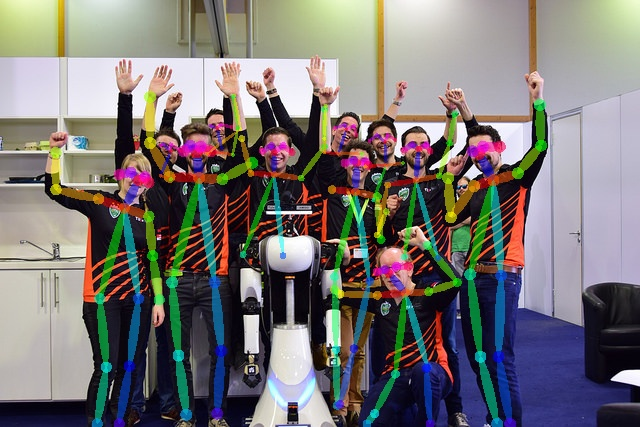
\includegraphics[width=0.66\linewidth]{openpose}
	\caption{Pose detection}
	\label{fig:pose_detection}
\end{figure} 

\section{Sound source localization}
To perform proper speech recognition, the direction of the sound is important to capture the sound source properly. We localize the sound source by determining the direction of arrival (DOA) with use of the microphone array board with 8 microphones\footnote{\url{https://creator.matrix.one}} of the Matrix Creator.
%depicted in Figure \ref{fig:matrix_one}.
%\begin{figure}[h]
%    \centering
%    %\vspace{-0.3cm}
%	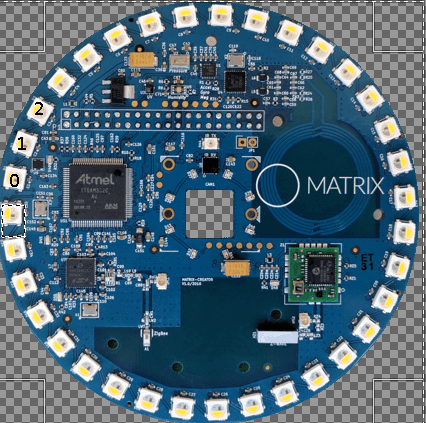
\includegraphics[width = 0.5\linewidth]{Figures/ssl_Matrix_creator.png}
%    %\vspace{-1em}
%	\caption{Matrix One Creator board.}
%	\label{fig:matrix_one}
%    %\vspace{-0.5cm}
%\end{figure}
The detection is done by first calculating the time cross correlation between four pairs of opposing microphones. Second, the microphone pair with the lowest phase shift w.r.t. the opposing microphone is selected as being perpendicular to the source. Finally, the direction of the source can be determined by combining this information with the energy level\footnote{\url{https://github.com/tue-robotics/matrix-creator-hal}} of the microphones. Our software for the DOA detection is available on GitHub, as well as a ROS package\footnote{\url{https://github.com/tue-robotics/matrix_creator_ros}} that exposes the DOA detections via a geometry\_msgs/PoseStamped topic interface. 

%\subsection{Reasoning}
%The reasoning layer of the AMIGO ROS based software consists of a set of finite state machines (robot\_smach\_states\footnote{\url{https://github.com/tue-robotics/robot_smach_states}}) that build upon the robot’s skill layer (robot\_skills\footnote{\url{https://github.com/tue-robotics/robot_skills}}). These state machines are useful if you want the robot to execute some complex plan, where all possible states and state transitions can be described explicitly. The implementation is done with use of the open-source SMACH package. %SMACH is a task-level architecture for rapidly creating complex robot behaviours. 

%\newpage
\section{Human-Robot Interface}
\label{ssec:webgui}
In order to interact with the robot, apart from speech, we have designed a web-based \gls{gui}. This interface uses HTML5\footnote{\url{https://github.com/tue-robotics/tue_mobile_ui}} with the Robot API written in Javascript and we host it on the robot itself.
%This allows multiple users on different platforms (\eg\ Android, iOS) to access functionalities of the robot. The interface is implemented in JavaScript with AngularJS and it offers a graphical interface to the Robot API\footnote{\url{https://github.com/tue-robotics/robot-api}} which exposes all the functionality of the robot.
%\begin{figure}[h]
%    \centering
%	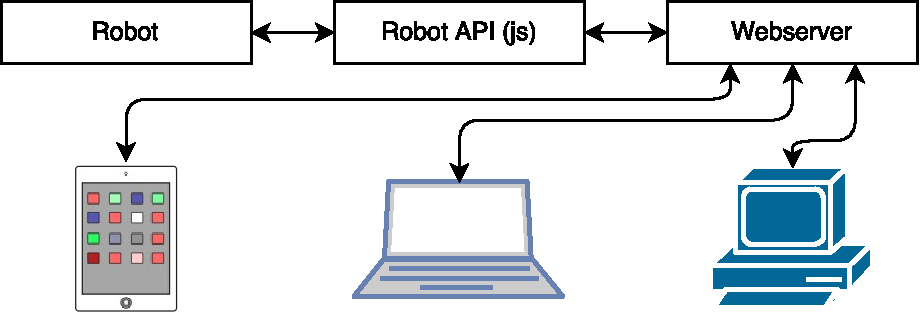
\includegraphics[width=0.9\linewidth]{Figures/webgui_architecture}
%    %\vspace{-0.5em}
%	\caption{
%		Overview of the WebGUI architecture.
%		A webserver that is hosting the \protect\gls{gui} connects this %Robot API to a graphical interface that is offered to multiple clients on %different platforms.}
%	\label{fig:webgui_architecture}
%\end{figure}
%Figure~\ref{fig:gui_actions} gives an example of various user interactions that are possible with the \gls{gui} and the different commands that can be given to the robot while interacting with the virtual scene.

\begin{figure}[H]
	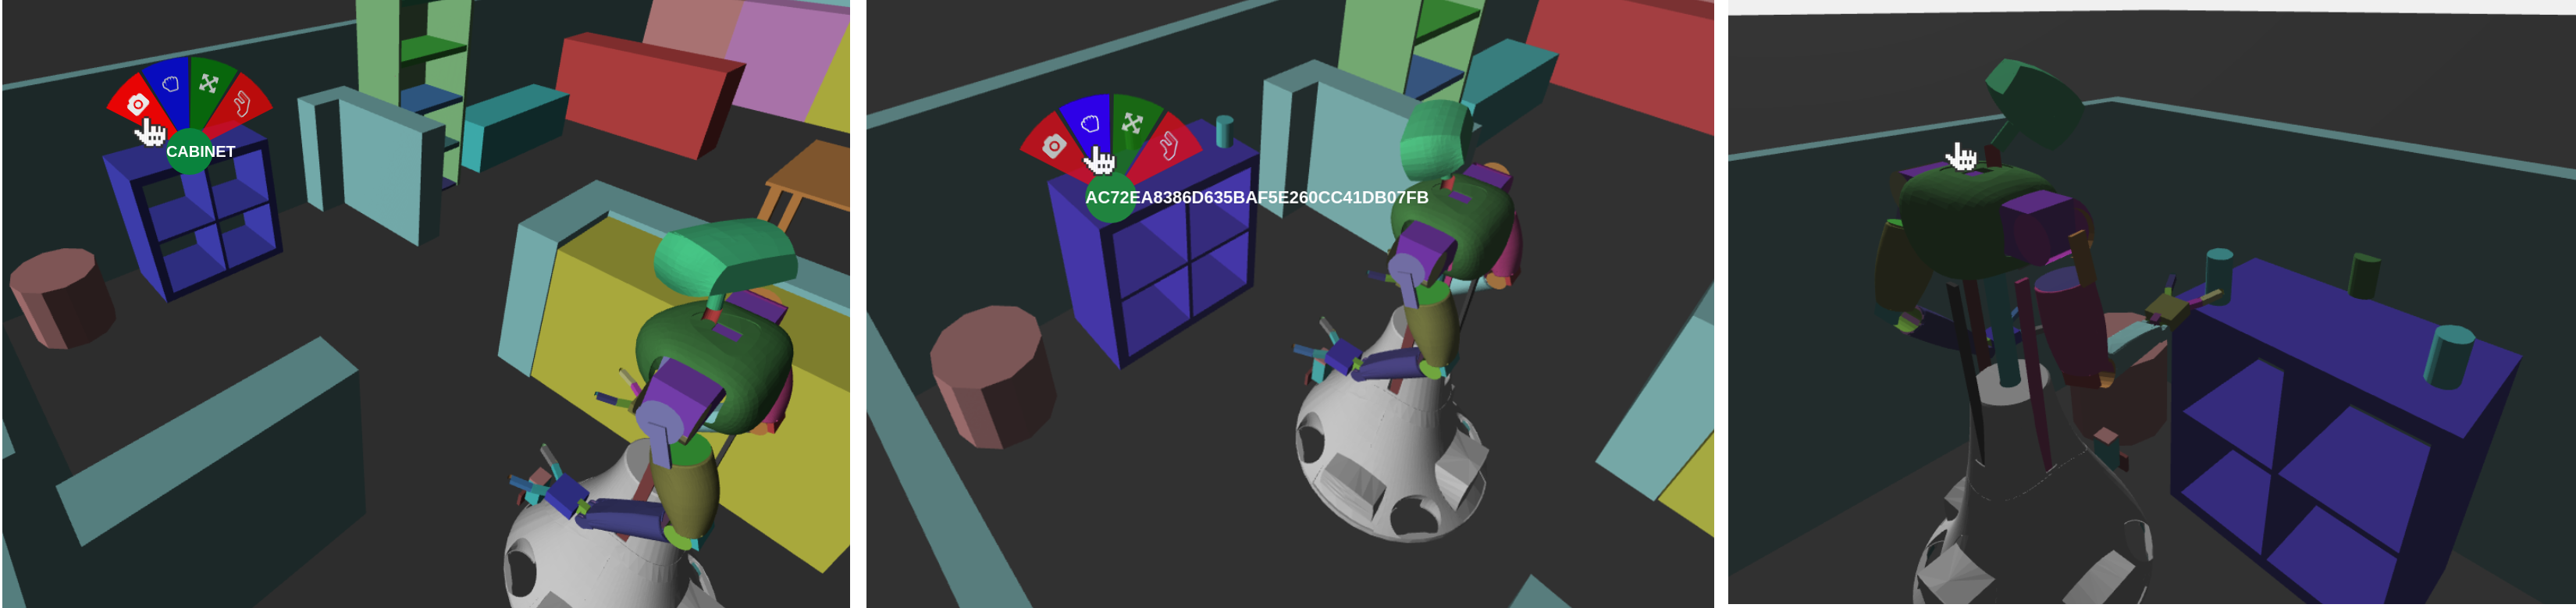
\includegraphics[width=\linewidth]{Figures/gui_actions}
	\caption{
		Illustration of the 3D scene of the WebGUI with AMIGO.
		User can long-press objects to open a menu from which actions on the object can be triggered
%		Users can interact with use of the menu that appears when long pressing an object in the scene.
%		On the left figure, the user commands the robot to inspect the selected object, which is the `cabinet'.
%		When the robot has inspected the `cabinet', it has found entities on top of it.
%		In the middle figure a grasp command is given to the robot to pick up an object from the cabinet.
%		The last figure show the robot executing that action.
		}
	\label{fig:gui_actions}

\end{figure}
%Figure \ref{fig:webgui_architecture} gives an overview of the connections between these components and 
\noindent Figure \ref{fig:gui_actions} represents an instance of the various interactions that are possible with the Robot API.



\subsection{Re-usability of the system for other research groups}
Tech United takes great pride in creating and maintaining open-source software and hardware to accelerate innovation. Tech United initiated the Robotic Open Platform website\footnote{\url{http://roboticopenplatform.org/}}, to share hardware designs. All packages are equipped with documentation and tutorials. Tech United and its scientific staff have the capacity to co-develop (+10 people), maintain and assist with questions

\subsection{Community Outreach and Media}
The Tech United team carries out many promotional activities for children to promote technology and innovation. These activities are performed by separate teams of student assistants. Tech United often visits primary and secondary schools, public events, trade fairs and has regular TV appearances. In 2015 and 2016 combined, 100+ demos were given and an estimated 50k people were reached through live interaction.
Tech United also has a very active website\footnote{\url{http://www.techunited.nl}}, and interacts on many social media like: Facebook\footnote{\url{https://www.facebook.com/techunited}}, YouTube\footnote{\url{https://www.youtube.com/user/TechUnited}}, Twitter\footnote{\url{https://www.twitter.com/TechUnited}} and Flickr\footnote{\url{https://www.flickr.com/photos/techunited/}}. Our robotics videos are often shared on the IEEE video Friday website. 


%%%%%%%%%%%%%%%%%%%%%%%%%%%%%%%%%%%%%%%%%%%%%%%%%%%%%%%%%%%%%%%%%%%%%%%%%%%%%%%%%%%%%
%%
%% Bibliography\usepackage{graphicx}
%%
%%%%%%%%%%%%%%%%%%%%%%%%%%%%%%%%%%%%%%%%%%%%%%%%%%%%%%%%%%%%%%%%%%%%%%%%%%%%%%%%%%%%%

\section*{Bibliography}
\bibliographystyle{unsrt}
\bibliography{refs}

%%%%%%%%%%%%%%%%%%%%%%%%%%%%%%%%%%%%%%%%%%%%%%%%%%%%%%%%%%%%%%%%%%%%%%%%%%%%%%%%%%%%%
%%
%% Robot Specifications
%%
%%%%%%%%%%%%%%%%%%%%%%%%%%%%%%%%%%%%%%%%%%%%%%%%%%%%%%%%%%%%%%%%%%%%%%%%%%%%%%%%%%%%%
%
\robospecs
%\newpage
%%\section*{HSR's Software and External Devices}
% In this section briefly describe the software and hardware of the robot

\setlength\intextsep{0pt}
\begin{wrapfigure}[5]{r}{0.3\textwidth}
	\centering
	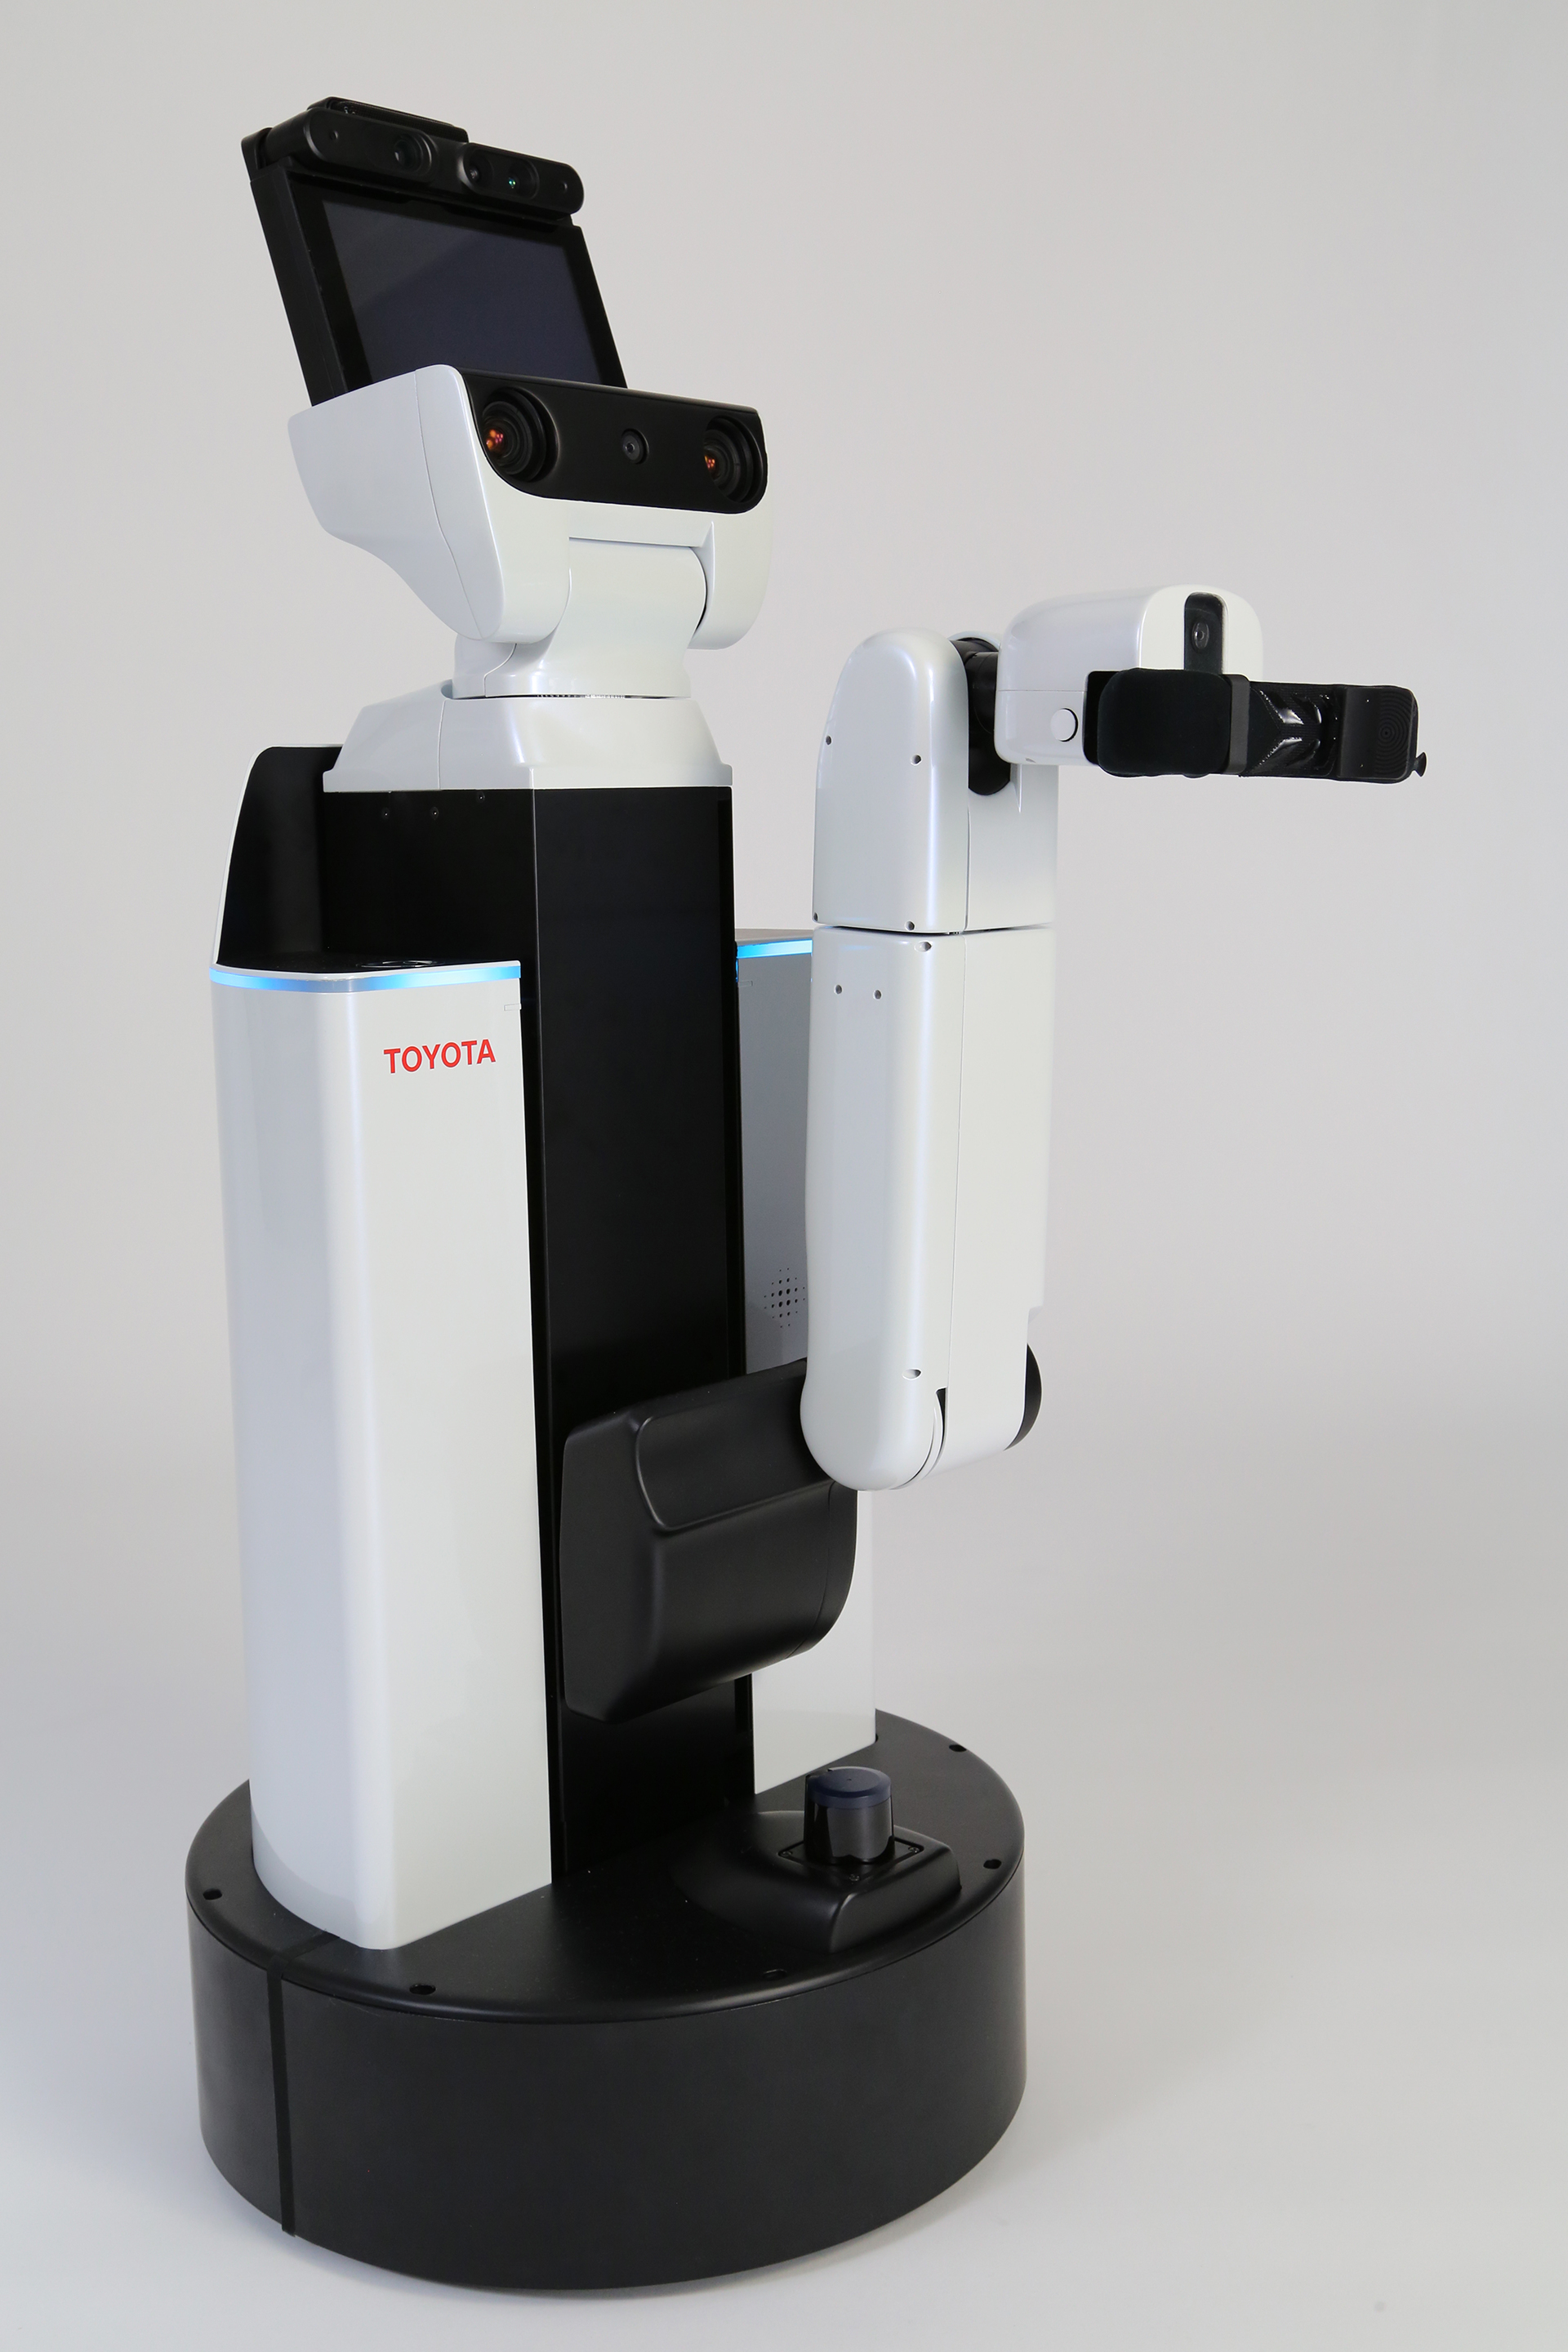
\includegraphics[width=0.3\textwidth]{Toyota_HSR}
	\caption{The Toyota HSR Robot, HERO}
	\label{fig:hsr}
\end{wrapfigure}

We use a standard \textit{Toyota} HSR robot unit. To differentiate our unit, we named it HERO. We wanted to link the name to our AMIGO and SERGIO domestic service robots.

\section*{HERO's Software Description}
% Please describe in this section the software you are using to control your robot. Consider the following example:

An overview of the software used by the Tech United Eindhoven @Home robots can be found in Table~\ref{tab:softwarespec}.
All our software is developed open-source at GitHub\footnote{\url{https://github.com/tue-robotics}}.
\\\newline
Currently, we have some \textit{image\_recognition} packages released into the current ROS Kinetic distribution and can be installed with use of \textit{apt}.

\begin{table}[H]
    \begin{center}
    \caption{Software overview of the robots.}
    \label{tab:softwarespec}
    %\vspace{-0.1cm}
    \renewcommand{\arraystretch}{1.0}
    \setlength{\tabcolsep}{5pt}
        \begin{tabular}{p{0.3\textwidth} p{0.7\textwidth}}
            \toprule
            Operating system & Ubuntu 16.04 LTS Server\\

            Middleware & ROS Kinetic~\cite{Quigley2009}\\

            Low-level control software & Orocos Real-Time Toolkit~\cite{Bruyninckx2001}\newline
            \url{https://github.com/tue-robotics/rtt_control_components}
            \\

            Simulation & Custom kinematics + sensor simulator \newline
            \url{https://github.com/tue-robotics/fast_simulator}
            \\

            World model & \acrfull{ed}, custom \newline
            \url{https://github.com/tue-robotics/ed}\\

            Localization & Monte Carlo~\cite{Fox2003} using \gls{ed}, custom \newline \url{https://github.com/tue-robotics/ed\_localization}\\

            SLAM & Gmapping package \newline \url{http://wiki.ros.org/gmapping}\\

            Navigation & CB Base navigation
            \newline
            \url{https://github.com/tue-robotics/cb_base_navigation}
            \newline
            Global: custom A* planner\newline Local: modified ROS DWA~\cite{Fox1997}\\

            Arm navigation & Custom implementation using MoveIt and Orocos KDL\newline
            \url{https://github.com/tue-robotics/tue_manipulation}
            \\

            Object recognition & Tensorflow ROS \newline
			\url{https://github.com/tue-robotics/image\_recognition/tree/master/tensorflow\_ros}\\

            People detection & Custom implementation using contour matching \newline
            \url{https://github.com/tue-robotics/ed_perception}
            \\
            Face detection \& recognition & Openface ROS \newline \url{https://github.com/tue-robotics/image\_recognition/tree/master/openface\_ros} \\

            Speech recognition & Julius Speech Recognition \newline
            \url{https://github.com/julius-speech/julius}\\
            Speech synthesis & Toyota\texttrademark \hspace{0em} Text-to-Speech\\
            Task executors & SMACH \newline
            \url{https://github.com/tue-robotics/tue_robocup}\\
            \bottomrule
        \end{tabular}
    \end{center}
\end{table}

This our current software implementation on our robots AMIGO and SERGIO, which participate in the open league. Because of the pending delivery of the Toyota HSR and related documentation, we are not able to provide the specific software implementation. As described in our selection qualification paper, our goal is to use the same software as possible on all our robots, including the Toyota HSR.

\section*{External Devices}
% Please describe in this section the external devices used by your robot. Consider the following example:

\textit{HERO relies on the following external hardware:}

\begin{itemize}
	\item Mother-ship
	\item Data Cluster
	\item $3 \times$ Ultra-Power laptops.
\end{itemize}

\section*{Cloud Services}
% Please describe in this section the Cloud Services and online software used by your robot. Consider the following example:

\textit{HERO connects the following cloud services:}
\begin{itemize}
	\item Localization and mapping: Geolocalization system.
	\item Navigation: Navigator
	\item Speech recognition: All-purpose recognizer.
\end{itemize} 
\newpage
\section*{Amigo's Hardware Description}
% In this section briefly describe the software and hardware of the robot

\setlength\intextsep{0pt}
\begin{wrapfigure}[15]{r}{0.3\textwidth}
	\centering
	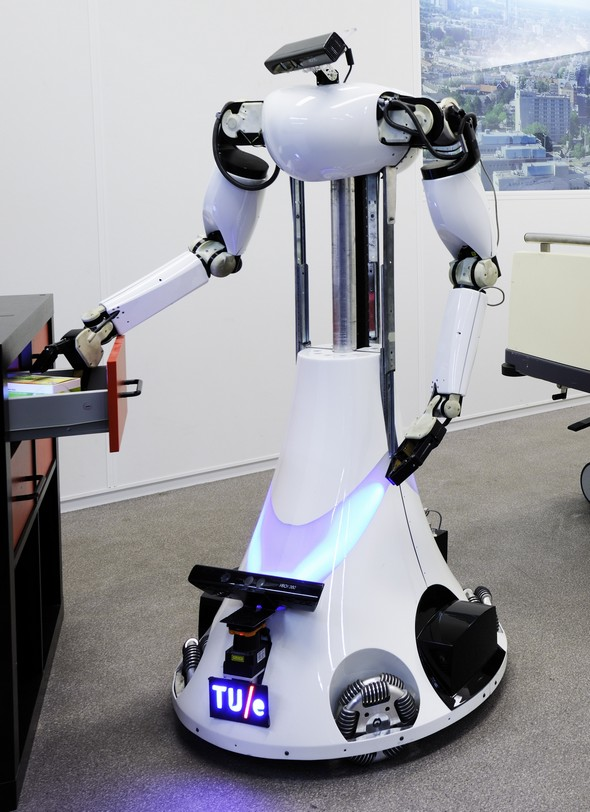
\includegraphics[width=0.3\textwidth]{amigo}
	\caption{The Amigo Robot}
	\label{fig:amigo}
\end{wrapfigure}

AMIGO (Autonomous Mate for Intelligent Operations, see Fig.~\ref{fig:amigo}) has competed in RoboCup@Home since 2011. Its design is based on a Middle Size League soccer robot, equipped with two Philips\texttrademark \hspace{0em} Experimental Robotic Arms mounted on an extensible upper body. Based on our experiences with AMIGO, SERGIO (Second Edition Robot for Generic Indoor Operations, has been developed. The main differences with AMIGO are the use of Mecanum wheels which are compliantly suspended, the torso with two degrees of freedom and the modular setup. The core specifications of AMIGO are shown in Table~\ref{tab:hardwarespec}. More details about the robots are on the Robotic Open Platform\footnote{\texttt{http://www.roboticopenplatform.org/}}, where all CAD drawings, electrical schematics and CAD files are published. SERGIO will not enter the competition this year. \\

\begin{table}[H]
    \begin{center}
    \caption{Core specifications of AMIGO}
    \label{tab:hardwarespec}
    \renewcommand{\arraystretch}{1.0}
    \setlength{\tabcolsep}{5pt}
        \begin{tabular}{p{0.2\textwidth} p{0.4\textwidth}}
            \toprule
            & AMIGO \\
            \midrule
            Name & Autonomous Mate for IntelliGent Operations \\
            Base & Fully holonomic omni-wheel platform  \\
            Torso & 1 vertical DoF using a ball screw \\
            Manipulators & 2 7-DoF Philips\texttrademark \hspace{0em} Experimental Robotic Arms \\
            Neck & Pan-tilt unit using two Dynamixel RX-64 servo actuators \\
            Head & Microsoft Kinect\texttrademark \hspace{0em} for XBox 360\texttrademark \\
            External devices & Wireless emergency button \\
            Dimensions & Diameter: $0.75\ \mathrm{m}$, height: $\pm1.5\ \mathrm{m}$ \\
            Weight & $\pm84\ \mathrm{kg}$ \\
            Additional sensors & Hokuyo UTM-30LX laser range finder on base and torso\\
            Microphone & R{\O}DE Videomic and Matrix Creator\\
            Batteries & $4\times$ Makita $24\ \mathrm{V},\ 3.3\ \mathrm{Ah}$ \\
            Computers & $3\times$ AOpen Mini PC with Core-i7 processor and $8\ \mathrm{GB}$ RAM and NVidia Jetson TX2 \\
            \bottomrule
        \end{tabular}
    \end{center}
\end{table}

\newpage
\section*{Amigo's Software Description}
% Please describe in this section the software you are using to control your robot. Consider the following example:

An overview of the software used by the Tech United Eindhoven @Home robots is shown in Table~\ref{tab:softwarespec}.
All our software is developed open-source on GitHub\footnote{\url{https://github.com/tue-robotics}}.
\\\newline
Some \textit{image\_recognition} packages are released into the ROS Kinetic distribution and can be installed with use of \textit{apt}.\\


\begin{table}[H]
    \begin{center}
    \caption{Software overview of Amigo.}
    \label{tab:softwarespec}
    %\vspace{-0.1cm}
    \renewcommand{\arraystretch}{1.0}
    \setlength{\tabcolsep}{5pt}
        \begin{tabular}{p{0.3\textwidth} p{0.7\textwidth}}
            \toprule
            Operating system & Ubuntu 16.04 LTS Server\\

            Middleware & ROS Kinetic~\cite{Quigley2009}\\

            Low-level control software & Orocos Real-Time Toolkit~\cite{Bruyninckx2001}\newline
            \url{https://github.com/tue-robotics/rtt_control_components}
            \\

            Simulation & Custom kinematics + sensor simulator \newline
            \url{https://github.com/tue-robotics/fast_simulator}
            \\

            World model & \acrfull{ed}, custom \newline
            \url{https://github.com/tue-robotics/ed}\\

            Localization & Monte Carlo~\cite{Fox2003} using \gls{ed}, custom \newline \url{https://github.com/tue-robotics/ed_localization}\\

            SLAM & Gmapping package \newline \url{http://wiki.ros.org/gmapping}\\

            Navigation & CB Base navigation
            \newline
            \url{https://github.com/tue-robotics/cb_base_navigation}
            \newline
            Global: custom A* planner\newline Local: modified ROS DWA~\cite{Fox1997}\\

            Arm navigation & Custom implementation using MoveIt and Orocos KDL\newline
            \url{https://github.com/tue-robotics/tue_manipulation}
            \\

            Object recognition & Tensorflow ROS \newline
			\url{https://github.com/tue-robotics/image_recognition/tree/master/tensorflow_ros}\\

            People detection & Custom implementation using contour matching \newline
            \url{https://github.com/tue-robotics/ed_perception}
            \\
            Face detection \& recognition & Openface ROS \newline \url{https://github.com/tue-robotics/image_recognition/tree/master/openface_ros} \\

            Speech recognition & Dragonfly + Windows\texttrademark \hspace{0em} Speech Recognition \newline
            \url{https://github.com/tue-robotics/dragonfly_speech_recognition}\\
            Speech synthesis & \texttrademark \hspace{0em} Text-to-Speech\\
            Task executors & SMACH \newline
            \url{https://github.com/tue-robotics/tue_robocup}\\
            \bottomrule
        \end{tabular}
    \end{center}
\end{table}

\section*{External Devices}
% Please describe in this section the external devices used by your robot. Consider the following example:
TODO: Update this page!\\

\textit{Amigo relies on the following external hardware:}

\begin{itemize}
	\item  Wireless emergency stop
	\item  etc.
\end{itemize}

\section*{Cloud Services}
% Please describe in this section the Cloud Services and online software used by your robot. Consider the following example:

\textit{Amigo connects the following cloud services:}
\begin{itemize}
	\item Localization and mapping:
    \item Speech recognition:
    \item etc.
\end{itemize} 



\end{document}
